% Options for packages loaded elsewhere
% Options for packages loaded elsewhere
\PassOptionsToPackage{unicode}{hyperref}
\PassOptionsToPackage{hyphens}{url}
\PassOptionsToPackage{dvipsnames,svgnames,x11names}{xcolor}
%
\documentclass[
  russian,
]{article}
\usepackage{xcolor}
\usepackage[top=20mm,left=20mm,right=20mm,bottom=20mm]{geometry}
\usepackage{amsmath,amssymb}
\setcounter{secnumdepth}{5}
\usepackage{iftex}
\ifPDFTeX
  \usepackage[T1]{fontenc}
  \usepackage[utf8]{inputenc}
  \usepackage{textcomp} % provide euro and other symbols
\else % if luatex or xetex
  \usepackage{unicode-math} % this also loads fontspec
  \defaultfontfeatures{Scale=MatchLowercase}
  \defaultfontfeatures[\rmfamily]{Ligatures=TeX,Scale=1}
\fi
\usepackage{lmodern}
\ifPDFTeX\else
  % xetex/luatex font selection
  \setmainfont[]{Times New Roman}
  \setsansfont[]{Arial}
  \setmonofont[]{Courier New}
\fi
% Use upquote if available, for straight quotes in verbatim environments
\IfFileExists{upquote.sty}{\usepackage{upquote}}{}
\IfFileExists{microtype.sty}{% use microtype if available
  \usepackage[]{microtype}
  \UseMicrotypeSet[protrusion]{basicmath} % disable protrusion for tt fonts
}{}
\makeatletter
\@ifundefined{KOMAClassName}{% if non-KOMA class
  \IfFileExists{parskip.sty}{%
    \usepackage{parskip}
  }{% else
    \setlength{\parindent}{0pt}
    \setlength{\parskip}{6pt plus 2pt minus 1pt}}
}{% if KOMA class
  \KOMAoptions{parskip=half}}
\makeatother
% Make \paragraph and \subparagraph free-standing
\makeatletter
\ifx\paragraph\undefined\else
  \let\oldparagraph\paragraph
  \renewcommand{\paragraph}{
    \@ifstar
      \xxxParagraphStar
      \xxxParagraphNoStar
  }
  \newcommand{\xxxParagraphStar}[1]{\oldparagraph*{#1}\mbox{}}
  \newcommand{\xxxParagraphNoStar}[1]{\oldparagraph{#1}\mbox{}}
\fi
\ifx\subparagraph\undefined\else
  \let\oldsubparagraph\subparagraph
  \renewcommand{\subparagraph}{
    \@ifstar
      \xxxSubParagraphStar
      \xxxSubParagraphNoStar
  }
  \newcommand{\xxxSubParagraphStar}[1]{\oldsubparagraph*{#1}\mbox{}}
  \newcommand{\xxxSubParagraphNoStar}[1]{\oldsubparagraph{#1}\mbox{}}
\fi
\makeatother


\usepackage{longtable,booktabs,array}
\newcounter{none} % for unnumbered tables
\usepackage{calc} % for calculating minipage widths
% Correct order of tables after \paragraph or \subparagraph
\usepackage{etoolbox}
\makeatletter
\patchcmd\longtable{\par}{\if@noskipsec\mbox{}\fi\par}{}{}
\makeatother
% Allow footnotes in longtable head/foot
\IfFileExists{footnotehyper.sty}{\usepackage{footnotehyper}}{\usepackage{footnote}}
\makesavenoteenv{longtable}
\usepackage{graphicx}
\makeatletter
\newsavebox\pandoc@box
\newcommand*\pandocbounded[1]{% scales image to fit in text height/width
  \sbox\pandoc@box{#1}%
  \Gscale@div\@tempa{\textheight}{\dimexpr\ht\pandoc@box+\dp\pandoc@box\relax}%
  \Gscale@div\@tempb{\linewidth}{\wd\pandoc@box}%
  \ifdim\@tempb\p@<\@tempa\p@\let\@tempa\@tempb\fi% select the smaller of both
  \ifdim\@tempa\p@<\p@\scalebox{\@tempa}{\usebox\pandoc@box}%
  \else\usebox{\pandoc@box}%
  \fi%
}
% Set default figure placement to htbp
\def\fps@figure{htbp}
\makeatother



\ifLuaTeX
\usepackage[bidi=basic,shorthands=off,provide=*]{babel}
\else
\usepackage[bidi=default,shorthands=off,provide=*]{babel}
\fi
\ifPDFTeX
\else
\babelfont{rm}[]{Times New Roman}
\fi
\ifLuaTeX
  \usepackage{selnolig} % disable illegal ligatures
\fi


\setlength{\emergencystretch}{3em} % prevent overfull lines

\providecommand{\tightlist}{%
  \setlength{\itemsep}{0pt}\setlength{\parskip}{0pt}}



 


\makeatletter
\@ifpackageloaded{tcolorbox}{}{\usepackage[skins,breakable]{tcolorbox}}
\@ifpackageloaded{fontawesome5}{}{\usepackage{fontawesome5}}
\definecolor{quarto-callout-color}{HTML}{909090}
\definecolor{quarto-callout-note-color}{HTML}{0758E5}
\definecolor{quarto-callout-important-color}{HTML}{CC1914}
\definecolor{quarto-callout-warning-color}{HTML}{EB9113}
\definecolor{quarto-callout-tip-color}{HTML}{00A047}
\definecolor{quarto-callout-caution-color}{HTML}{FC5300}
\definecolor{quarto-callout-color-frame}{HTML}{acacac}
\definecolor{quarto-callout-note-color-frame}{HTML}{4582ec}
\definecolor{quarto-callout-important-color-frame}{HTML}{d9534f}
\definecolor{quarto-callout-warning-color-frame}{HTML}{f0ad4e}
\definecolor{quarto-callout-tip-color-frame}{HTML}{02b875}
\definecolor{quarto-callout-caution-color-frame}{HTML}{fd7e14}
\makeatother
\makeatletter
\@ifpackageloaded{caption}{}{\usepackage{caption}}
\AtBeginDocument{%
\ifdefined\contentsname
  \renewcommand*\contentsname{Содержание}
\else
  \newcommand\contentsname{Содержание}
\fi
\ifdefined\listfigurename
  \renewcommand*\listfigurename{Список Иллюстраций}
\else
  \newcommand\listfigurename{Список Иллюстраций}
\fi
\ifdefined\listtablename
  \renewcommand*\listtablename{Список Таблиц}
\else
  \newcommand\listtablename{Список Таблиц}
\fi
\ifdefined\figurename
  \renewcommand*\figurename{Рисунок}
\else
  \newcommand\figurename{Рисунок}
\fi
\ifdefined\tablename
  \renewcommand*\tablename{Таблица}
\else
  \newcommand\tablename{Таблица}
\fi
}
\@ifpackageloaded{float}{}{\usepackage{float}}
\floatstyle{ruled}
\@ifundefined{c@chapter}{\newfloat{codelisting}{h}{lop}}{\newfloat{codelisting}{h}{lop}[chapter]}
\floatname{codelisting}{Список}
\newcommand*\listoflistings{\listof{codelisting}{Список Каталогов}}
\makeatother
\makeatletter
\makeatother
\makeatletter
\@ifpackageloaded{caption}{}{\usepackage{caption}}
\@ifpackageloaded{subcaption}{}{\usepackage{subcaption}}
\makeatother
\usepackage{bookmark}
\IfFileExists{xurl.sty}{\usepackage{xurl}}{} % add URL line breaks if available
\urlstyle{same}
% fallback for those not using the hyperref driver hyperxmp:
\makeatletter
\@ifundefined{xmpquote}{\newcommand{\xmpquote}[1]{#1}}{}
\makeatother
\hypersetup{
  pdftitle={Задачи по Эконометрике-1: Метод наименьших квадратов},
  pdfauthor={Н. В. Артамонов, А. Н. Лата (МГИМО МИД России)},
  pdflang={ru},
  colorlinks=true,
  linkcolor={blue},
  filecolor={Maroon},
  citecolor={Blue},
  urlcolor={Blue},
  pdfcreator={LaTeX via pandoc}}


\title{Задачи по Эконометрике-1: Метод наименьших квадратов}
\author{Н. В. Артамонов, А. Н. Лата (МГИМО МИД России)}
\date{}
\begin{document}
\maketitle

\renewcommand*\contentsname{Содержание}
{
\setcounter{tocdepth}{3}
\tableofcontents
}

\section{Теория}\label{ux442ux435ux43eux440ux438ux44f}

\subsection{Задача (прямая с
константой)}\label{ux437ux430ux434ux430ux447ux430-ux43fux440ux44fux43cux430ux44f-ux441-ux43aux43eux43dux441ux442ux430ux43dux442ux43eux439}

Пусть задано \(n\) наблюдений (точек на плоскости)
\(\lbrace x_i,y_i\rbrace_{i=1}^n\). Линейная функция
\(y=\beta_0+\beta_1x\) «подгоняется» под наблюдения методом наименьших
квадратов (OLS):

\begin{itemize}
\tightlist
\item
  выведите систему уравнений для нахождения параметров оптимальной
  (подогнанной) прямой, наименее уклоняющейся от заданных наблюдений;
\item
  выведите формулы для оценок \(\widehat{\beta}_0\) и
  \(\widehat{\beta}_1\) коэффициентов оптимальной прямой;
\item
  покажите, что для оценок коэффициентов верно:
\end{itemize}

\[
\begin{aligned}
  \widehat{\beta}_1&=\frac{\mathrm{s.cov}(x,y)}{\mathrm{s.Var}(x)}, &
  \widehat{\beta}_0&=\bar{y}-\widehat{\beta}_1\cdot \bar{x}.
\end{aligned}
\]

Здесь \(\mathrm{s.cov}(x,y)\) --- выборочная ковариация,
\(\mathrm{s.Var}(x)\) --- выборочная дисперсия.

\subsection{Задача (прямая без
константы)}\label{ux437ux430ux434ux430ux447ux430-ux43fux440ux44fux43cux430ux44f-ux431ux435ux437-ux43aux43eux43dux441ux442ux430ux43dux442ux44b}

Пусть задано \(n\) наблюдений (точек на плоскости)
\(\lbrace x_i,y_i\rbrace_{i=1}^n\). Линейная функция \(y=\beta x\)
подгоняется под наблюдения методом наименьших квадратов (OLS):

\begin{itemize}
\tightlist
\item
  выведите уравнение для нахождения параметра оптимальной прямой,
  наименее уклоняющейся от заданных наблюдений (точек на плоскости);
\item
  выведите формулу для оценки \(\widehat{\beta}\) коэффициента
  оптимальной прямой.
\end{itemize}

\subsection{Задача (обратная регрессия без
константы)}\label{ux437ux430ux434ux430ux447ux430-ux43eux431ux440ux430ux442ux43dux430ux44f-ux440ux435ux433ux440ux435ux441ux441ux438ux44f-ux431ux435ux437-ux43aux43eux43dux441ux442ux430ux43dux442ux44b}

Пусть \(\widehat{\beta}\) есть OLS-оценка коэффициента наклона линейной
функции \(y\) на \(x\) без константы, а \(\widehat{\gamma}\) ---
OLS-оценка коэффициента наклона линейной функции \(x\) на \(y\) без
константы. Верно ли для этих оценок равенство

\[
\widehat{\gamma}=\frac{1}{\widehat{\beta}}?
\]

Ответ поясните.

\subsection{Задача (обратная регрессия с
константой)}\label{ux437ux430ux434ux430ux447ux430-ux43eux431ux440ux430ux442ux43dux430ux44f-ux440ux435ux433ux440ux435ux441ux441ux438ux44f-ux441-ux43aux43eux43dux441ux442ux430ux43dux442ux43eux439}

Пусть \(\widehat{\beta}_1\) есть OLS-оценка коэффициента наклона
линейной функции \(y\) на \(x\) с константой, а \(\widehat{\gamma}_1\)
--- OLS-оценка коэффициента наклона линейной функции \(x\) на \(y\) с
константой. Верно ли равенство

\[
\widehat{\gamma}_1=\frac{1}{\widehat{\beta}_1}?
\]

Ответ поясните.

\subsection{Задача (квадратичный
многочлен)}\label{ux437ux430ux434ux430ux447ux430-ux43aux432ux430ux434ux440ux430ux442ux438ux447ux43dux44bux439-ux43cux43dux43eux433ux43eux447ux43bux435ux43d}

Пусть задано \(n\) наблюдений (точек на плоскости)
\(\lbrace x_i,y_i\rbrace_{i=1}^n\). Парабола
\(y=\beta_0+\beta_1x+\beta_2x^2\) подгоняется под наблюдения методом
наименьших квадратов (OLS). Выведите систему уравнений для нахождения
параметров оптимальной параболы.

\section{Практика
(Python)}\label{ux43fux440ux430ux43aux442ux438ux43aux430-python}

\begin{tcolorbox}[enhanced jigsaw, arc=.35mm, bottomrule=.15mm, bottomtitle=1mm, breakable, colback=white, colbacktitle=quarto-callout-important-color!10!white, colframe=quarto-callout-important-color-frame, coltitle=black, left=2mm, leftrule=.75mm, opacityback=0, opacitybacktitle=0.6, rightrule=.15mm, title=\textcolor{quarto-callout-important-color}{\faExclamation}\hspace{0.5em}{Важно}, titlerule=0mm, toprule=.15mm, toptitle=1mm]

\begin{itemize}
\tightlist
\item
  Во всех задачах логарифм натуральный; константа включается по
  умолчанию.
\item
  Данные --- в папке \texttt{datasets/}, описание наборов данных --- в
  файле
  \href{../datasets/data-description.md}{\texttt{datasets/data-description.md}}.
\item
  Численные ответы округлите до 2-х десятичных знаков; оценки, которые
  при этом обращаются в ноль, --- до трёх значащих цифр.
\item
  В ответах коэффициенты подписаны так, как их выводит statsmodels:
  \texttt{Intercept} --- константа, \texttt{np.log(x)} --- \(\log x\),
  \texttt{I(x\ **\ 2)} --- \(x^2\).
\end{itemize}

\end{tcolorbox}

\subsection{sleep equation \#1}\label{sleep-equation-1}

Для набора данных \texttt{sleep75} (\texttt{sleep}, \texttt{totwrk} ---
минуты в неделю, \texttt{age} --- годы) рассмотрим регрессию
\textbf{sleep на totwrk}.

Постройте диаграмму рассеяния \textbf{sleep vs totwrk} с подогнанной
прямой.

Ответ: Рисунок~\ref{fig-sleep-totwrk}; на нём показаны обе прямые --- с
константой и без константы.

\begin{figure}

\centering{

\pandocbounded{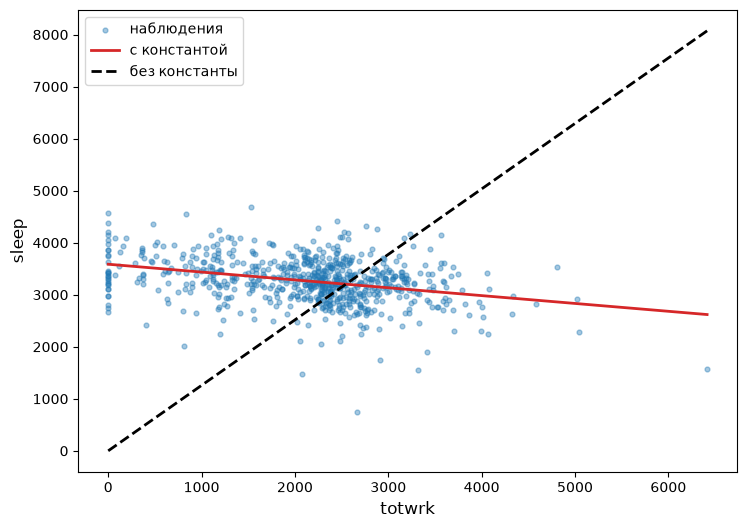
\includegraphics[keepaspectratio]{list01-OLS_files/figure-pdf/fig-sleep-totwrk-output-1.png}}

}

\caption{\label{fig-sleep-totwrk}sleep и totwrk: подогнанные прямые с
константой и без константы}

\end{figure}%

\textbf{С константой}

Найдите параметры оптимальной прямой \textbf{sleep на totwrk}.
\textbf{Ответ округлите до 2-х десятичных знаков.}

Ответ:

{\def\LTcaptype{none} % do not increment counter
\begin{longtable}[]{@{}lr@{}}
\toprule\noalign{}
Переменная & Оценка \\
\midrule\noalign{}
\endhead
\bottomrule\noalign{}
\endlastfoot
Intercept & 3586.38 \\
totwrk & -0.15 \\
\end{longtable}
}

Модель была подогнана по 706 наблюдениям.

\textbf{Без константы}

Найдите параметры оптимальной прямой \textbf{sleep на totwrk} без
константы. \textbf{Ответ округлите до 2-х десятичных знаков.}

Ответ:

{\def\LTcaptype{none} % do not increment counter
\begin{longtable}[]{@{}lr@{}}
\toprule\noalign{}
Переменная & Оценка \\
\midrule\noalign{}
\endhead
\bottomrule\noalign{}
\endlastfoot
totwrk & 1.26 \\
\end{longtable}
}

Модель была подогнана по 706 наблюдениям.

\subsection{sleep equation \#2}\label{sleep-equation-2}

Для набора данных \texttt{sleep75} рассмотрим регрессию \textbf{sleep на
age}.

Постройте диаграмму рассеяния \textbf{sleep vs age} с подогнанной
прямой.

Ответ: Рисунок~\ref{fig-sleep-age}; на нём показаны обе прямые --- с
константой и без константы.

\begin{figure}

\centering{

\pandocbounded{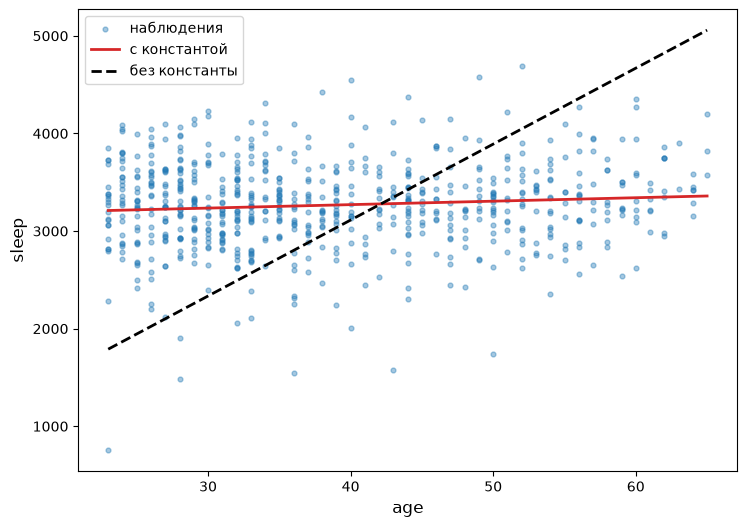
\includegraphics[keepaspectratio]{list01-OLS_files/figure-pdf/fig-sleep-age-output-1.png}}

}

\caption{\label{fig-sleep-age}sleep и age: подогнанные прямые с
константой и без константы}

\end{figure}%

\textbf{С константой}

Найдите параметры оптимальной прямой \textbf{sleep на age}.
\textbf{Ответ округлите до 2-х десятичных знаков.}

Ответ:

{\def\LTcaptype{none} % do not increment counter
\begin{longtable}[]{@{}lr@{}}
\toprule\noalign{}
Переменная & Оценка \\
\midrule\noalign{}
\endhead
\bottomrule\noalign{}
\endlastfoot
Intercept & 3128.91 \\
age & 3.54 \\
\end{longtable}
}

Модель была подогнана по 706 наблюдениям.

\textbf{Без константы}

Найдите параметры оптимальной прямой \textbf{sleep на age} без
константы. \textbf{Ответ округлите до 2-х десятичных знаков.}

Ответ:

{\def\LTcaptype{none} % do not increment counter
\begin{longtable}[]{@{}lr@{}}
\toprule\noalign{}
Переменная & Оценка \\
\midrule\noalign{}
\endhead
\bottomrule\noalign{}
\endlastfoot
age & 77.82 \\
\end{longtable}
}

Модель была подогнана по 706 наблюдениям.

\subsection{sleep equation \#3}\label{sleep-equation-3}

Для набора данных \texttt{sleep75} рассмотрим регрессию \textbf{sleep на
totwrk, I(totwrk**2)}.

Постройте диаграмму рассеяния \textbf{sleep vs totwrk} с подогнанной
параболой.

Ответ: Рисунок~\ref{fig-sleep-totwrk-sq}.

\begin{figure}

\centering{

\pandocbounded{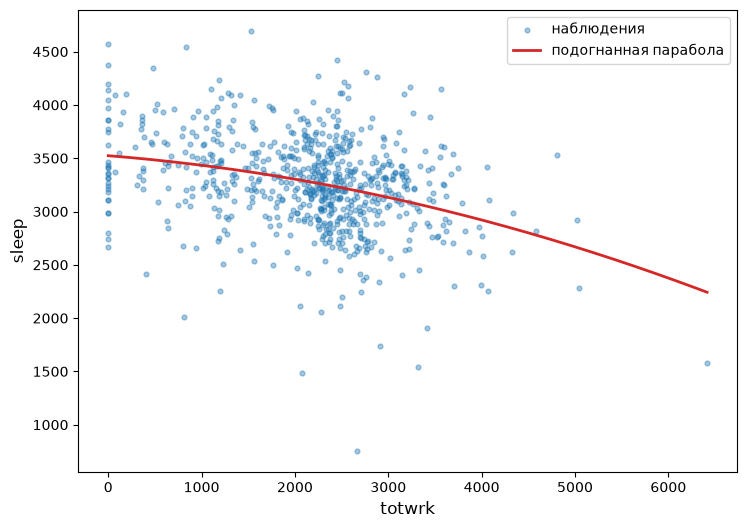
\includegraphics[keepaspectratio]{list01-OLS_files/figure-pdf/fig-sleep-totwrk-sq-output-1.png}}

}

\caption{\label{fig-sleep-totwrk-sq}sleep и totwrk: подогнанная
парабола}

\end{figure}%

Найдите параметры оптимальной параболы \textbf{sleep на totwrk,
I(totwrk**2)}. \textbf{Ответ округлите до 2-х десятичных знаков.}

Ответ:

{\def\LTcaptype{none} % do not increment counter
\begin{longtable}[]{@{}lr@{}}
\toprule\noalign{}
Переменная & Оценка \\
\midrule\noalign{}
\endhead
\bottomrule\noalign{}
\endlastfoot
Intercept & 3523.59 \\
totwrk & -0.07 \\
I(totwrk ** 2) & -2.03e-05 \\
\end{longtable}
}

Модель была подогнана по 706 наблюдениям.

\subsection{sleep equation \#4}\label{sleep-equation-4}

Для набора данных \texttt{sleep75} рассмотрим регрессию \textbf{sleep на
age, I(age**2)}.

Постройте диаграмму рассеяния \textbf{sleep vs age} с подогнанной
параболой.

Ответ: Рисунок~\ref{fig-sleep-age-sq}.

\begin{figure}

\centering{

\pandocbounded{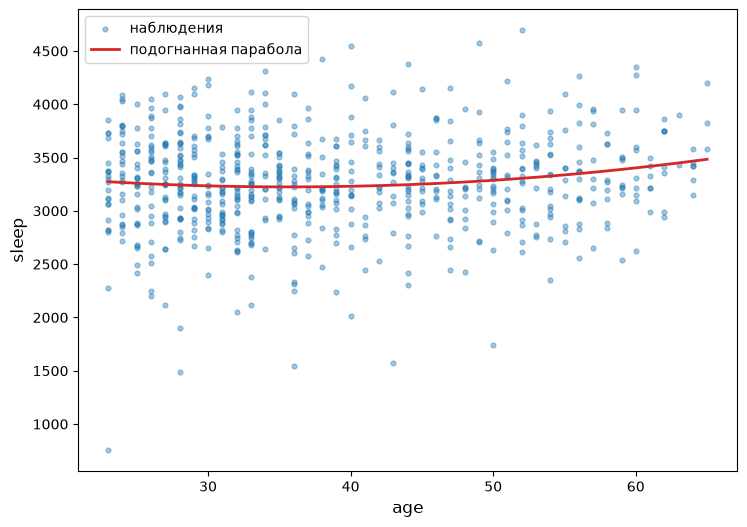
\includegraphics[keepaspectratio]{list01-OLS_files/figure-pdf/fig-sleep-age-sq-output-1.png}}

}

\caption{\label{fig-sleep-age-sq}sleep и age: подогнанная парабола}

\end{figure}%

Найдите параметры оптимальной параболы \textbf{sleep на age, I(age**2)}.
\textbf{Ответ округлите до 2-х десятичных знаков.}

Ответ:

{\def\LTcaptype{none} % do not increment counter
\begin{longtable}[]{@{}lr@{}}
\toprule\noalign{}
Переменная & Оценка \\
\midrule\noalign{}
\endhead
\bottomrule\noalign{}
\endlastfoot
Intercept & 3608.03 \\
age & -21.49 \\
I(age ** 2) & 0.30 \\
\end{longtable}
}

Модель была подогнана по 706 наблюдениям.

\subsection{sleep equation \#5}\label{sleep-equation-5}

Для набора данных \texttt{sleep75} рассмотрим регрессию \textbf{sleep на
totwrk, age}.

Найдите параметры оптимальной плоскости \textbf{sleep на totwrk, age}.
\textbf{Ответ округлите до 2-х десятичных знаков.}

Ответ:

{\def\LTcaptype{none} % do not increment counter
\begin{longtable}[]{@{}lr@{}}
\toprule\noalign{}
Переменная & Оценка \\
\midrule\noalign{}
\endhead
\bottomrule\noalign{}
\endlastfoot
Intercept & 3469.20 \\
totwrk & -0.15 \\
age & 2.92 \\
\end{longtable}
}

Модель была подогнана по 706 наблюдениям.

\subsection{output equation \#1}\label{output-equation-1}

Для набора данных \texttt{Labour} (\texttt{output}, \texttt{capital} ---
млн евро, \texttt{labour} --- число работников) рассмотрим регрессии
\textbf{output на capital} и \textbf{np.log(output) на np.log(capital)}.

\textbf{Гистограммы}

Постройте гистограммы переменных \textbf{output, np.log(output),
capital, np.log(capital), labour, np.log(labour)}.

Ответ: Рисунок~\ref{fig-labour-hist}.

\begin{figure}

\centering{

\pandocbounded{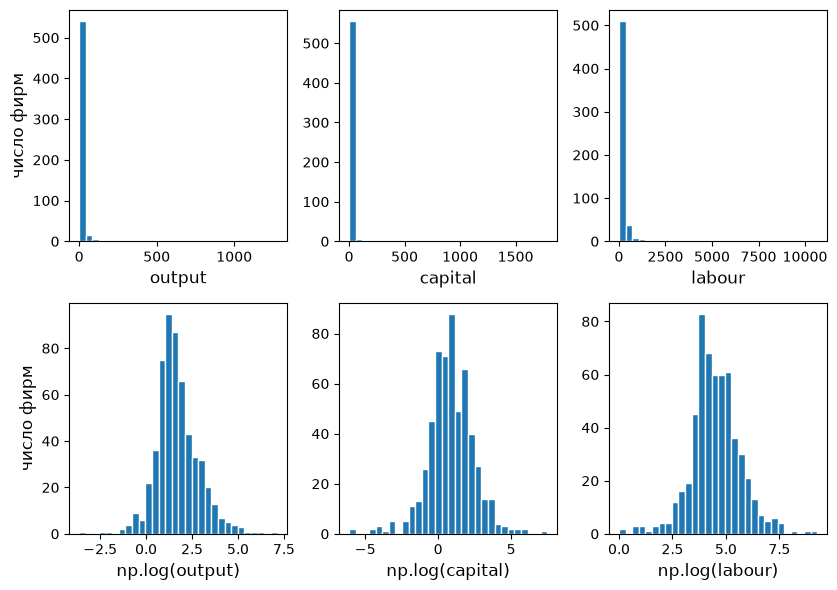
\includegraphics[keepaspectratio]{list01-OLS_files/figure-pdf/fig-labour-hist-output-1.png}}

}

\caption{\label{fig-labour-hist}Гистограммы output, capital, labour и их
логарифмов (Labour)}

\end{figure}%

\textbf{Диаграмма рассеяния}

Постройте диаграмму рассеяния \textbf{output vs capital} с подогнанной
прямой.

Ответ: Рисунок~\ref{fig-output-capital}; на нём показаны обе прямые ---
с константой и без константы.

\begin{figure}

\centering{

\pandocbounded{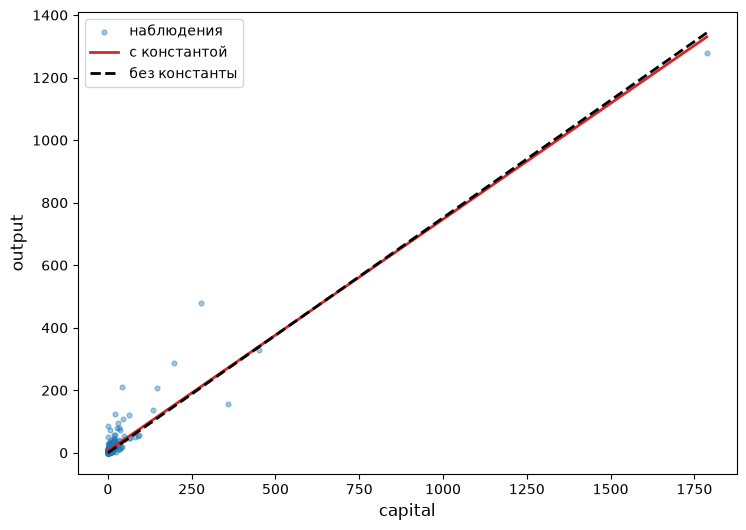
\includegraphics[keepaspectratio]{list01-OLS_files/figure-pdf/fig-output-capital-output-1.png}}

}

\caption{\label{fig-output-capital}output и capital: подогнанные прямые
с константой и без константы}

\end{figure}%

\textbf{С константой}

Найдите параметры оптимальной прямой \textbf{output на capital}.
\textbf{Ответ округлите до 2-х десятичных знаков.}

Ответ:

{\def\LTcaptype{none} % do not increment counter
\begin{longtable}[]{@{}lr@{}}
\toprule\noalign{}
Переменная & Оценка \\
\midrule\noalign{}
\endhead
\bottomrule\noalign{}
\endlastfoot
Intercept & 6.19 \\
capital & 0.74 \\
\end{longtable}
}

Модель была подогнана по 569 наблюдениям.

\textbf{Без константы}

Найдите параметры оптимальной прямой \textbf{output на capital} без
константы. \textbf{Ответ округлите до 2-х десятичных знаков.}

Ответ:

{\def\LTcaptype{none} % do not increment counter
\begin{longtable}[]{@{}lr@{}}
\toprule\noalign{}
Переменная & Оценка \\
\midrule\noalign{}
\endhead
\bottomrule\noalign{}
\endlastfoot
capital & 0.75 \\
\end{longtable}
}

Модель была подогнана по 569 наблюдениям.

\textbf{Диаграмма рассеяния в логарифмах}

Постройте диаграмму рассеяния \textbf{np.log(output) vs np.log(capital)}
с подогнанной прямой.

Ответ: Рисунок~\ref{fig-output-capital-log}; на нём показаны обе прямые
--- с константой и без константы.

\begin{figure}

\centering{

\pandocbounded{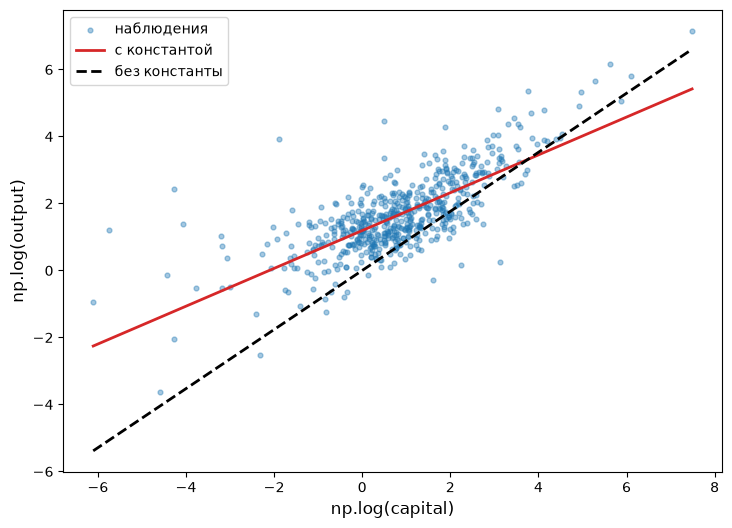
\includegraphics[keepaspectratio]{list01-OLS_files/figure-pdf/fig-output-capital-log-output-1.png}}

}

\caption{\label{fig-output-capital-log}np.log(output) и np.log(capital):
подогнанные прямые с константой и без константы}

\end{figure}%

\textbf{В логарифмах, с константой}

Найдите параметры оптимальной прямой \textbf{np.log(output) на
np.log(capital)}. \textbf{Ответ округлите до 2-х десятичных знаков.}

Ответ:

{\def\LTcaptype{none} % do not increment counter
\begin{longtable}[]{@{}lr@{}}
\toprule\noalign{}
Переменная & Оценка \\
\midrule\noalign{}
\endhead
\bottomrule\noalign{}
\endlastfoot
Intercept & 1.19 \\
np.log(capital) & 0.56 \\
\end{longtable}
}

Модель была подогнана по 569 наблюдениям.

\textbf{В логарифмах, без константы}

Найдите параметры оптимальной прямой \textbf{np.log(output) на
np.log(capital)} без константы. \textbf{Ответ округлите до 2-х
десятичных знаков.}

Ответ:

{\def\LTcaptype{none} % do not increment counter
\begin{longtable}[]{@{}lr@{}}
\toprule\noalign{}
Переменная & Оценка \\
\midrule\noalign{}
\endhead
\bottomrule\noalign{}
\endlastfoot
np.log(capital) & 0.88 \\
\end{longtable}
}

Модель была подогнана по 569 наблюдениям.

\subsection{output equation \#2}\label{output-equation-2}

Для набора данных \texttt{Labour} рассмотрим регрессии \textbf{output на
labour} и \textbf{np.log(output) на np.log(labour)}.

\textbf{Диаграмма рассеяния}

Постройте диаграмму рассеяния \textbf{output vs labour} с подогнанной
прямой.

Ответ: Рисунок~\ref{fig-output-labour}; на нём показаны обе прямые --- с
константой и без константы.

\begin{figure}

\centering{

\pandocbounded{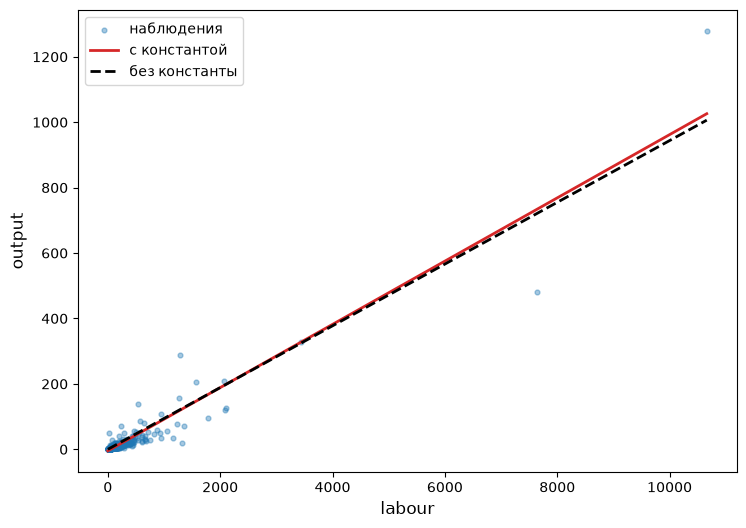
\includegraphics[keepaspectratio]{list01-OLS_files/figure-pdf/fig-output-labour-output-1.png}}

}

\caption{\label{fig-output-labour}output и labour: подогнанные прямые с
константой и без константы}

\end{figure}%

\textbf{С константой}

Найдите параметры оптимальной прямой \textbf{output на labour}.
\textbf{Ответ округлите до 2-х десятичных знаков.}

Ответ:

{\def\LTcaptype{none} % do not increment counter
\begin{longtable}[]{@{}lr@{}}
\toprule\noalign{}
Переменная & Оценка \\
\midrule\noalign{}
\endhead
\bottomrule\noalign{}
\endlastfoot
Intercept & -4.72 \\
labour & 0.10 \\
\end{longtable}
}

Модель была подогнана по 569 наблюдениям.

\textbf{Без константы}

Найдите параметры оптимальной прямой \textbf{output на labour} без
константы. \textbf{Ответ округлите до 2-х десятичных знаков.}

Ответ:

{\def\LTcaptype{none} % do not increment counter
\begin{longtable}[]{@{}lr@{}}
\toprule\noalign{}
Переменная & Оценка \\
\midrule\noalign{}
\endhead
\bottomrule\noalign{}
\endlastfoot
labour & 0.09 \\
\end{longtable}
}

Модель была подогнана по 569 наблюдениям.

\textbf{Диаграмма рассеяния в логарифмах}

Постройте диаграмму рассеяния \textbf{np.log(output) vs np.log(labour)}
с подогнанной прямой.

Ответ: Рисунок~\ref{fig-output-labour-log}; на нём показаны обе прямые
--- с константой и без константы.

\begin{figure}

\centering{

\pandocbounded{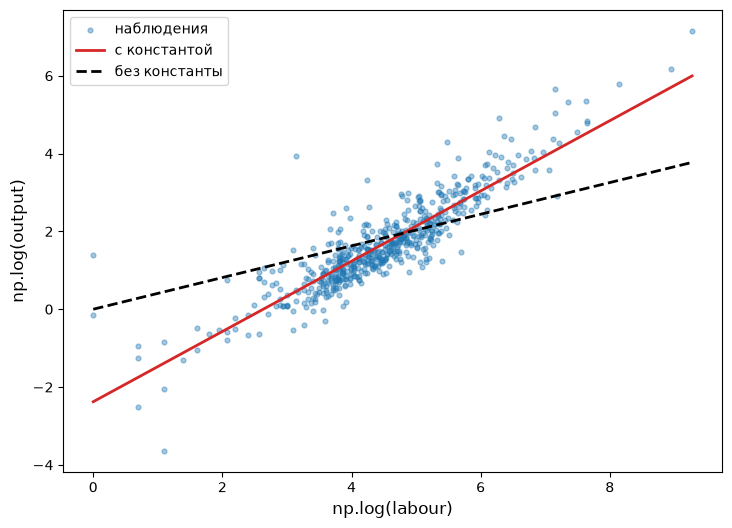
\includegraphics[keepaspectratio]{list01-OLS_files/figure-pdf/fig-output-labour-log-output-1.png}}

}

\caption{\label{fig-output-labour-log}np.log(output) и np.log(labour):
подогнанные прямые с константой и без константы}

\end{figure}%

\textbf{В логарифмах, с константой}

Найдите параметры оптимальной прямой \textbf{np.log(output) на
np.log(labour)}. \textbf{Ответ округлите до 2-х десятичных знаков.}

Ответ:

{\def\LTcaptype{none} % do not increment counter
\begin{longtable}[]{@{}lr@{}}
\toprule\noalign{}
Переменная & Оценка \\
\midrule\noalign{}
\endhead
\bottomrule\noalign{}
\endlastfoot
Intercept & -2.38 \\
np.log(labour) & 0.90 \\
\end{longtable}
}

Модель была подогнана по 569 наблюдениям.

\textbf{В логарифмах, без константы}

Найдите параметры оптимальной прямой \textbf{np.log(output) на
np.log(labour)} без константы. \textbf{Ответ округлите до 2-х десятичных
знаков.}

Ответ:

{\def\LTcaptype{none} % do not increment counter
\begin{longtable}[]{@{}lr@{}}
\toprule\noalign{}
Переменная & Оценка \\
\midrule\noalign{}
\endhead
\bottomrule\noalign{}
\endlastfoot
np.log(labour) & 0.41 \\
\end{longtable}
}

Модель была подогнана по 569 наблюдениям.

\subsection{output equation \#3}\label{output-equation-3}

Для набора данных \texttt{Labour} рассмотрим регрессию
\textbf{np.log(output) на np.log(capital), I(np.log(capital)**2)}.

Постройте диаграмму рассеяния \textbf{np.log(output) vs np.log(capital)}
с подогнанной параболой.

Ответ: Рисунок~\ref{fig-output-capital-sq}.

\begin{figure}

\centering{

\pandocbounded{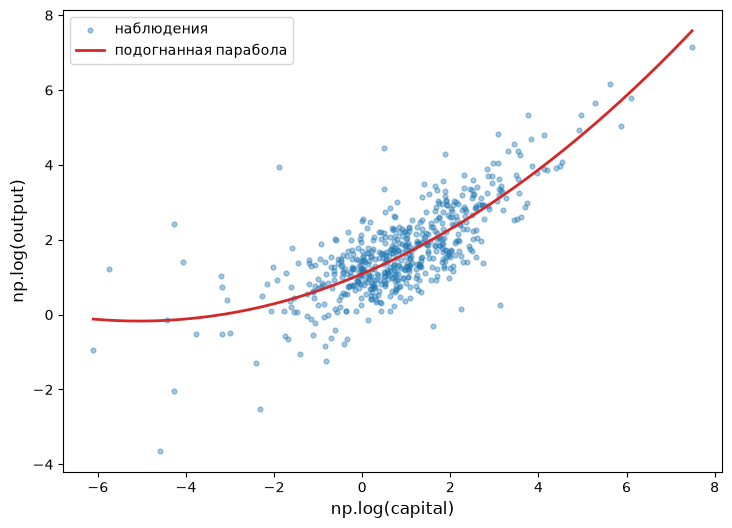
\includegraphics[keepaspectratio]{list01-OLS_files/figure-pdf/fig-output-capital-sq-output-1.png}}

}

\caption{\label{fig-output-capital-sq}np.log(output) и np.log(capital):
подогнанная парабола}

\end{figure}%

Найдите параметры оптимальной параболы \textbf{np.log(output) на
np.log(capital), I(np.log(capital)**2)}. \textbf{Ответ округлите до 2-х
десятичных знаков.}

Ответ:

{\def\LTcaptype{none} % do not increment counter
\begin{longtable}[]{@{}lr@{}}
\toprule\noalign{}
Переменная & Оценка \\
\midrule\noalign{}
\endhead
\bottomrule\noalign{}
\endlastfoot
Intercept & 1.09 \\
np.log(capital) & 0.50 \\
I(np.log(capital) ** 2) & 0.05 \\
\end{longtable}
}

Модель была подогнана по 569 наблюдениям.

\subsection{output equation \#4}\label{output-equation-4}

Для набора данных \texttt{Labour} рассмотрим регрессию
\textbf{np.log(output) на np.log(labour), I(np.log(labour)**2)}.

Постройте диаграмму рассеяния \textbf{np.log(output) vs np.log(labour)}
с подогнанной параболой.

Ответ: Рисунок~\ref{fig-output-labour-sq}.

\begin{figure}

\centering{

\pandocbounded{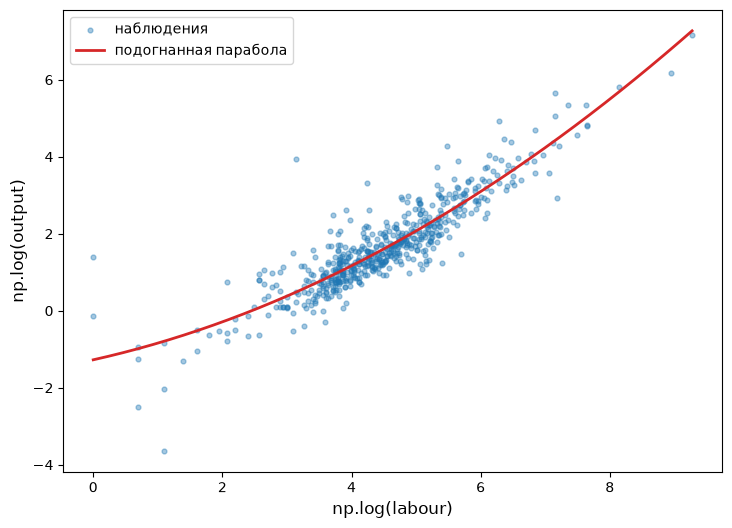
\includegraphics[keepaspectratio]{list01-OLS_files/figure-pdf/fig-output-labour-sq-output-1.png}}

}

\caption{\label{fig-output-labour-sq}np.log(output) и np.log(labour):
подогнанная парабола}

\end{figure}%

Найдите параметры оптимальной параболы \textbf{np.log(output) на
np.log(labour), I(np.log(labour)**2)}. \textbf{Ответ округлите до 2-х
десятичных знаков.}

Ответ:

{\def\LTcaptype{none} % do not increment counter
\begin{longtable}[]{@{}lr@{}}
\toprule\noalign{}
Переменная & Оценка \\
\midrule\noalign{}
\endhead
\bottomrule\noalign{}
\endlastfoot
Intercept & -1.28 \\
np.log(labour) & 0.37 \\
I(np.log(labour) ** 2) & 0.06 \\
\end{longtable}
}

Модель была подогнана по 569 наблюдениям.




\end{document}
